\id{МРНТИ 65.59.29}{}

\begin{articleheader}
\sectionwithauthors{Г.Е. Исламова, А.А. Утебаева, А.У.Шингисов}{Изучение органолептических характеристик и жирнокислотного состава мясного хлеба, обогащённого томатными выжимками}

{\bfseries
Г.Е. Исламова\textsuperscript{\envelope },
А.А. Утебаева,
А.У.Шингисов
}
\end{articleheader}

\begin{affiliation}
Южно-Казахстанский университет им. М. Ауэзова, Шымкент, Казахстан,

\raggedright \textsuperscript{\envelope }Корреспондент-автор: Gulnura\_87\_KZ@mail.ru
\end{affiliation}

В данной работе исследуется влияние порошка из томатного жмыха (ПТЖ) на
органолептические характеристики и жирнокислотный состав мясного хлеба.
Актуальность исследования обусловлена растущим интересом к
функциональным продуктам питания, обогащённым растительными
компонентами, а также необходимостью рационального использования пищевых
отходов.

В ходе исследования были подготовлены образцы мясного хлеба с различным
содержанием ПТЖ (10\%, 15\% и 20\%) и проведена их органолептическая
оценка по пятибалльной гедонистической шкале. Оптимальный уровень
добавления ПТЖ составил 15\%, что обеспечило улучшение вкусовых и
цветовых характеристик, не нарушая традиционной структуры мясного
продукта. При этом отмечено повышение насыщенности цвета, усиление
аромата и улучшение текстуры по сравнению с контрольным образцом.

Анализ жирнокислотного состава методом газовой хроматографии показал,
что введение ПТЖ способствует увеличению содержания полиненасыщенных
жирных кислот, в частности линолевой и олеиновой кислот, а также
снижению уровня насыщенных жиров. Таким образом, применение томатных
выжимок не только повышает питательную ценность мясного хлеба, но и
способствует улучшению его функциональных свойств.

Полученные результаты подтверждают перспективность использования ПТЖ в
производстве мясных изделий, обеспечивая повышение их пищевой ценности,
органолептической привлекательности и экологической устойчивости
производства.

{\bfseries Ключевые слова}: функциональная добавка, мясной продукт, порошок
из томатных выжимок, мясной хлеб, органолептические показатели,
жирнокислотный состав

\begin{articleheader}
{\bfseries STUDY OF ORGANOLEPTIC CHARACTERISTICS AND FATTY ACID COMPOSITION
OF MEAT BREAD ENRICHED WITH TOMATO EXTRACTS}

{\bfseries
G.E. Islamova\textsuperscript{\envelope },
A.A. Utebaeva,
A.U.Shingisov
}
\end{articleheader}

\begin{affiliation}
South Kazakhstan University named after M. Auezov, Shymkent, Kazakhstan,

e-mail: Gulnura\_87\_KZ@mail.ru
\end{affiliation}

This paper examines the effect of tomato pomace powder (TPP) on the
organoleptic characteristics and fatty acid composition of meatloaf. The
relevance of the study is due to the growing interest in functional
foods enriched with plant components, as well as the need for rational
use of food waste.

During the study, meat loaf samples with different TPP content (10\%,
15\% and 20\%) were prepared and their organoleptic evaluation was
carried out on a nine-point hedonic scale. The optimal level of TPP
addition was 15\%, which ensured improvement of taste and color
characteristics without violating the traditional structure of the meat
produc.At the same time, an increase in color saturation, an increase in
aroma and an improvement in texture were noted compared to the control
sample.

Analysis of the fatty acid composition by gas chromatography (GC) showed
that the introduction of TPP contributes to an increase in the content
of polyunsaturated fatty acids, in particular linoleic and oleic acids,
as well as a decrease in the level of saturated fats.Thus, the use of
tomato pomace not only increases the nutritional value of meatloaf, but
also helps to improve its functional properties.

The obtained results confirm the prospects of using TPP in the
production of meat products, ensuring an increase in their nutritional
value, organoleptic appeal and environmental sustainability of
production.

{\bfseries Keywords}: functional additive,meat product, tomato pomace
powder, meat loaf, organoleptic properties, fatty acid composition

\begin{articleheader}
{\bfseries ҚЫЗАНАҚ СЫҒЫНДЫСЫМЕН БАЙЫТЫЛҒАН ЕТ НАНЫНЫҢ ОРГАНОЛЕПТИКАЛЫҚ СИПАТЫ ЖӘНЕ МАЙ ҚЫШҚЫЛДЫҚ ҚҰРАМЫН ЗЕРТТЕУ}

{\bfseries
Г.Е. Исламова\textsuperscript{\envelope },
А.А. Утебаева,
А.У.Шингисов
}
\end{articleheader}

\begin{affiliation}
М.Әуезов атындағы Оңтүстік Қазақстан университеті, Шымкент, Қазақстан,

e-mail: Gulnura\_87\_KZ@mail.ru
\end{affiliation}

Бұл жұмыста ет нанының органолептикалық көрсеткіштері мен май қышқылының
құрамын қызанақ ұнтағының әсері зерттелді. Зерттеудің өзектілігі өсімдік
компоненттері мен байытылған функционалдық тағамдарға деген
қызығушылықтың артуына, сондай-ақтамақ қалдықтарын ұтымды пайдалану
қажеттілігіне байланысты.

Зерттеу барысында ет нанының үлгілеріне әртүрлі мөлшердегі қызанақ
қалдығының ұнтағы (5\%, 10\%, 15\% және 20\%) дайындалып, олардың
органолептикалық бағалауы бес балдық гедоникалық шкала бойынша
жүргізілді. Қызанақ ұнтағын қосудың оңтайлы деңгейі 15\% құрады, бұл ет
өнімінің дәстүрлі құрылымын бұзбай,дәм мен түс сипаттамаларын жақсартуды
қамтамасыз етті..Бұл ретте бақылау үлгісімен салыстырғанда түсінің
қанықтылығының жоғарылауы, хош иістің күшеюі және текстураның жақсаруы
байқалды.

Газ хроматографиясы әдісімен май қышқылының құрамын талдау қызанақ
қалдығын қосу полиқанықпаған май қышқылдарының, атапайтқанда линол және
олеин қышқылдарының құрамын арттыруға, сондай-ақ қаныққан май деңгейін
төмендетуге ықпалететінін көрсетті. Осылайша, қызанақ қалдығын қолдану
ет нанының тағамдық құндылығын арттырып қана қоймайды, сонымен қатар
оның функционалдық қасиеттерін жақсартуға көмектеседі.

Алынған нәтижелер ет өнімдерін өндіруде қызанақ ұнтағын қолдану
перспективаларын растайды, олардың тағамдық құндылығын, органолептикалық
тартымдылығын және өндірістің экологиялық тұрақтылығын арттыруды
қамтамасыз етеді.

{\bfseries Түйін сөздер:} функционалдық қоспа, ет өнімі,қызанақ қалдығының
ұнтағы, ет наны, органолептикалық қасиеттері, май қышқылдарының құрамы

\begin{multicols}{2}
{\bfseries Введение.} Мясной хлеб является популярным мясным продуктом,
который традиционно готовят из мясного фарша, панировочных сухарей, яиц
и приправ. В последние годы повышенный интерес к функциональным
продуктам питания стимулирует исследования по улучшению его питательной
ценности за счёт включения растительных компонентов. Это нововведение не
только повышает пользу блюда для здоровья, но и вводит новые вкусы и
текстуры, делая его привлекательным для более широкой аудитории, включая
тех, кто стремится сократить потребление мяса {[}1,2{]}.

Потребители все чаще ищут функциональные продукты, которые предлагают
пользу для здоровья помимо основного питания. Согласно маркетинговым
исследованиям, ожидается, что мировой рынок функциональных продуктов
питания будет расти со среднегодовым темпом роста 8--10\% к 2030 году,
что обусловлено: ростом осведомленности о пищевых волокнах и
антиоксидантах, спросом на натуральные и экологически чистые
ингредиенты, растущей обеспокоенностью по поводу устойчивости продуктов
питания {[}3{]}.

Пищевые отходы являются серьезной проблемой: ежегодно 30--40 \% мирового
производства продуктов питания выбрасывается. Переработка томатов
приводит к образованию значительных побочных продуктов, включая кожуру и
семена, которые обычно выбрасываются или используются в качестве корма
для животных {[}4{]}.

В рамках устойчивого развития ученые и производители изучают возможность
превращения пищевых отходов в продукты с добавленной стоимостью,
сокращая отходы и одновременно улучшая питательные качества.

Таким образом, одним из перспективных направлений является обогащение
мясных изделий томатными выжимками -- побочным продуктом переработки
томатов, содержащим значительное количество биологически активных
соединений, включая ликопин, полифенолы и ненасыщенные жирные кислоты
{[}5, 6{]}.

Использование растительных добавок в мясных продуктах позволяет не
только повысить их пищевую ценность, но и улучшить органолептические
характеристики. Исследования показывают, что диета, обогащённая
томатными продуктами, может способствовать снижению риска
сердечно-сосудистых заболеваний за счёт положительного влияния на
липидный обмен {[}5, 6{]}.

Современные тенденции в пищевой промышленности направлены на создание
функциональных продуктов, способных оказывать благотворное влияние на
здоровье потребителей. В этом контексте особый интерес представляет
изменение липидного профиля мясных изделий за счёт включения
растительных компонентов, богатых ненасыщенными жирными кислотами.
Томатные выжимки могут способствовать увеличению содержания полезных
жирных кислот и снижению уровня насыщенных жиров, что актуально в
аспекте профилактики метаболических заболеваний.

Целью данного исследования является оценка влияния томатных выжимок на
органолептические характеристики и жирнокислотный состав мясного хлеба.
В работе анализируются сенсорные свойства продукта и изменения в его
липидном профиле при добавлении томатных выжимок.

Ряд исследований подтверждает эффективность применения растительных
порошков в мясной продукции {[}7,8{]}. В частности, использование
порошка томатных отходов обеспечивает сбалансированное питание, улучшает
цвет и вкус продукта без негативного влияния на его текстуру. В таблице
1 представлены основные преимущества и ограничения применения различных
овощных порошков в мясных продуктах.
\end{multicols}

\begin{longtblr}[
  caption = {\bfseries Таблица 1 - Применение овощных порошков в производстве мясных продуктов},
  label = none,
  entry = none,
]{
  width = \linewidth,
  colspec = {Q[158]Q[365]Q[225]Q[188]},
  cells = {c},
  hlines,
  vlines,
}
\textbf{Добавка} & \textbf{Основные			преимущества} & \textbf{Ограничения} & \textbf{Лучший			уровень использования, (\%)}\\
Порошок
			из томатных отходов (TWP) & Высокое
			содержание клетчатки, антиоксидантов,
			удержание влаги, натуральный красный
			цвет & Чрезмерное
			использование может повлиять на
			текстуру & 4–6\%\\
Морковный
			порошок & Добавляет
			β-каротин и натуральную сладость & Может
			слишком сильно смягчить текстуру & 3–5\%\\
Свекольный
			порошок & Сильный
			натуральный красный цвет, нитраты для
			здоровья сердца & Может
			перебить вкус & 2–4\%\\
Тыквенный
			порошок & Высокое
			содержание клетчатки и витамина А & Может
			значительно изменить текстуру мясного
			хлеба & 3–6\%\\
Яблочные
			выжимки & Улучшает
			удержание влаги и придает легкую
			сладость & Может
			сделать мясной рулет немного мягче & 3–7\%
\end{longtblr}

\begin{multicols}{2}
Ранее авторами данной работы были изучены методы переработки томатных
выжимок и их применение в мясных продуктах. Полученные результаты
подтверждают перспективность использования данной добавки для обогащения
мясного хлеба {[}9{]}. Кроме того, данные других исследований
свидетельствуют о высокой потребительской оценке мясных изделий с
томатными добавками по девятибалльной гедонистической шкале {[}10{]}.

Таким образом, использование томатных выжимок в производстве мясного
хлеба является перспективным направлением, сочетающим улучшение
питательной ценности, органолептических характеристик и повышение
экологической устойчивости пищевой промышленности.

{\bfseries Материалы и методы.} Объектами исследования являлись образцы
мясного хлеба с добавлением порошка из томатного жмыха в различных
концентрациях. Экспериментальные исследования проводились на базе
кафедры «Технология и безопасность продовольственных продуктов» ЮКУ им.
М. Ауэзова с применением стандартных общепринятых методик.
ГОСТ\,32951‑2014 «Полуфабрикаты мясные и мясосодержащие. Общие
технические условия». ISO 67.120.10 Meat and meat products.

В качестве растительной добавки в экспериментальном образце использовали
порошок, полученный из томатного жмыха. Свежий томатный жмых,
представляющий собой побочный продукт переработки томатов (содержащий
кожуру, семена и остатки мякоти), был предварительно просеян для
удаления крупных механических включений и затем гомогенизирован с
помощью лабораторного измельчителя до получения однородной массы. Сушка
жмыха проводилась в вакуум-сушильном шкафу при температуре 55\,±\,2\,°C
и остаточном давлении 20--25 кПа. Продолжительность сушки составляла 8
часов, до достижения остаточной массовой доли влаги не более 10\%. После
охлаждения до комнатной температуры высушенный жмых измельчали на
лабораторной мельнице до порошкообразного состояния. Средний размер
частиц полученного порошка не превышал 500 мкм. Готовый порошок хранился
в герметичных полиэтиленовых пакетах в сухом, тёмном помещении при
температуре (18--20\,°C).

Органолептическая оценка (цвет, вкус, аромат, консистенция) проводилась
методом пятибалльной гедонической шкалы.

Протокол органолептического тестирования

Наименование продукции: образцы мясного хлеба с добавлением порошка из
томатного жмыха в различных концентрациях; Дата проведения: 10.01.2025;
Место проведения: лаборатория кафедры «Технология и безопасность
продовольственных продуктов» ЮКУ им. М. Ауэзова; Количество образцов: 3
опытных образца + 1 контрольный; Количество повторов: 3 (каждому образцу
проводится оценка не менее чем в трёх повторах для повышения
достоверности результатов); Количество экспертов: 5.

Методика проведения

Образцы кодируются (например, A, B, C, D) и подаются в случайном
порядке. Каждый эксперт заполняет индивидуальный бланк оценки, выставляя
баллы по каждому показателю. Результаты по каждому образцу усредняются
по всем экспертам и по всем повторам. На основе полученных баллов
составляется рейтинг качества образцов.

Определение содержания метиловых эфиров жирных кислот (МЭЖК) выполнялось
методом газовой хроматографии (ГХ) на базе лаборатории АТУ. (Протокол №
9 от 15 января от 2025г).

Анализ жирнокислотного состава проводили методом газовой хроматографии.
Для подготовки проб липиды экстрагировали органическими растворителями с
методом сокслета с последующей метилированием триглицеридов с
использованием натрия метилата. Жирнокислотный анализ выполняли на
приборе газовой хроматограф "Кристаллюкс-400М" используя азот в качестве
газа-носителя. Тип колонки: Капиллярная колонка: HP-5 (5\% фенил, 95\%
метилполисилоксана). Размеры: длина 30 м, внутренний диаметр 0.25 мм,
толщина пленки 0.25 мкм. Скорость потока: 1.0 мл/мин (оптимально для
капиллярных колонок). Режим потока: постоянный поток (constant flow) -
обеспечивает стабильность времени удерживания. Температурный режим:
Температура испарителя: 230\,°C. Температура детектора ПИД: 250\,°C.
Программа температуры печи: Начальная температура: 50\,°C (удержание 2
мин), Подъём: 10\,°C/мин до 280\,°C, Удержание на конечной температуре:
5--10 мин. Объём вводимого образца: 1 мкл (при ручном или автоматическом
вводе). Сплит режим: Сплит-отношение 1:20 (или в зависимости от
концентрации анализируемого вещества).

Идентификацию жирных кислот проводили путем сравнения со стандартными
растворами жирных кислот ГОСТ Р 55483-2013.

{\bfseries Обсуждение и результаты.} В таблице 2 дана рецептура образцов
мясного хлеба -- контрольного и с концентрацией порошка из томатного
жмыха (ПТЖ) от 10\% до 20 \%. Подготовленные по разработанной нами
технологии и рецептуре образцы мясного хлеба с концентрацией порошка из
томатного жмыха (ПТЖ) от 10\% до 20 \% были исследованы по
органолептическим показателям (таблица 3, рисунок 1).
\end{multicols}

\begin{longtblr}[
  caption = {\bfseries Таблица 2 - Рецептура образцов мясного хлеба},
  label = none,
  entry = none,
]{
  cells = {c},
  hlines,
  vlines,
}
№ п\textbackslash{}п & Сырье,
			кг на 100 г сырья & {
			№1
			\\
			(контр)
		} & {
			Образец
			\\
			№1
			\\
			(10\%)
		} & {
			Образец
			\\
			№2
			\\
			(15\%)
		} & {
			Образец
			\\
			№3
			\\
			(20\%)
		}\\
1 & Баранина & 315 & 310 & 307,5 & 305\\
2 & Индейка & 315 & 310 & 307,5 & 305\\
3 & Яйца
			куриные & 120 & 120 & 120 & 120\\
4 & Лук
			репчатый свежий & 84 & 84 & 84 & 84\\
5 & Хлеб
			из пшеничной муки & 100 & 100 & 100 & 100\\
6 & Вода & 60 & 60 & 60 & 60\\
7 & Гималайская
			соль & 6 & 6 & 6 & 6\\
8 & Черный
			перец & 2 & 2 & 2 & 2\\
9 & Порошок
			томатного жмыха & - & 10 & 15 & 20
\end{longtblr}

\begin{longtblr}[
  caption = {\bfseries Таблица 3 - Органолептические показатели мясного хлеба в зависимости от содержания порошка из томатного жмыха (ПТЖ)},
  label = none,
  entry = none,
]{
  width = \linewidth,
  colspec = {Q[100]Q[123]Q[213]Q[283]Q[223]},
  cells = {c},
  hlines,
  vlines,
}
Наимено\-вание показа\-теля & Контроль & Образец № 1(10\%) & Образец № 2(15\%) & Образец № 3(20\%)\\
Конси\-стенция & Стандартная & Хорошая
			сочность, приятная текстура & Оптимальная
			мягкость и сочность & Плотная,
			слегка суховатая\\
Цвет & Обычный
			мясной & Легкий
			красноватый оттенок & Оптимальный
			насыщенный оттенок & Чрезмерно
			темный, красно-коричневый\\
Вкус & Чистый
			мясной & Легкий
			томатный привкус & Оптимальное
			сочетание мясного и томатного аромата & Чрезмерно
			выраженный аромат томатов\\
Аромат & Традицион\-ный
			мясной & Незначительный
			томатный аромат & Усиление
			натурального мясного аромата & Преобладание
			томатного аромата
\end{longtblr}

{\bfseries Риc.1 - Результаты балльной оценки органолептических
показателей мясного хлеба с разным содержанием ПТЖ}

Согласно данным рисунка 1, образец № 2(15\% ПТЖ) показал наилучшие
органолептические свойства, включая вкус, аромат и внешний вид -
оптимальное соотношение мясного и томатного компонентов. Контрольный
образец ожидаемо имеет традиционные характеристики. Образец №1 (10\%) -
достойный, но немного уступает по вкусу и аромату. Образец № 3(20\%) -
проигрывает из-за чрезмерной насыщенности томатного вкуса и плотной
текстуры.

Как известно, овощные добавки привносят новое измерение в сенсорные
ощущения от употребления мясного хлеба {[}11{]}.

Добавление порошка из томатного жмыха (ПТЖ) способствовало улучшению
цвета, внешнего вида и вкусового профиля, придавая мясному хлебу легкую
кислотность и делая его более сбалансированным по вкусу.

По результатам органолептической оценки можно сделать вывод, что
оптимальным является содержание ПТЖ на уровне 15\%, так как оно
способствует насыщенному красному оттенку, улучшает текстуру и усиливает
натуральные мясные и томатные ароматы. Каротиноиды в томатах играют
ключевую роль в формировании привлекательного цвета, снижая
необходимость использования искусственных красителей и усилителей вкуса.

Далее был определён жирнокислотный состав мясного хлеба с содержанием
порошка из томатного жмыха (ПТЖ) 15 \% в сравнении с контрольным
образцом. Полученные данные, отражающие влияние ПТЖ на липидный профиль
продукта, приведены в таблице 4 и на рисунках 2 и 3.

{\bfseries Таблица 4 - Жирнокислотный состав мясного хлеба с содержанием
порошка из томатного жмыха (ПТЖ) 15 \% в сравнении с контрольным
образцом}

%% \begin{longtable}[]{@{}
%%   >{\raggedright\arraybackslash}p{(\linewidth - 4\tabcolsep) * \real{0.3323}}
%%   >{\centering\arraybackslash}p{(\linewidth - 4\tabcolsep) * \real{0.3052}}
%%   >{\centering\arraybackslash}p{(\linewidth - 4\tabcolsep) * \real{0.3625}}@{}}
%% \toprule\noalign{}
%% \begin{minipage}[b]{\linewidth}\centering
%% {\bfseries Компонент}
%% \end{minipage} & \begin{minipage}[b]{\linewidth}\raggedright
%% {\bfseries Контрольный образец (концентрация, \% об.)}
%% \end{minipage} & \begin{minipage}[b]{\linewidth}\raggedright
%% {\bfseries Экспериментальный образец (15\%) (концентрация, \% об.)}
%% \end{minipage} \\
%% \midrule\noalign{}
%% \endhead
%% \bottomrule\noalign{}
%% \endlastfoot
%% Метилбутират & 2,173154 & 1,600267 \\
%% Метилгексаноат & 82,896302 & 56,987661 \\
%% Метиловый эфир цис-10-пентадеценовой кислоты & 0,015688 & 0,032050 \\
%% Метилпальмитолеат & 0,000116 & \\
%% Метилпальмитат & 0,002597 & 0,005663 \\
%% Метиловый эфир цис-10-гептадекановой кислоты & 0,000013 & 0,000033 \\
%% Метилгептадеканоат & 3,193092 & 8,124987 \\
%% Метиловый эфир γ-линоленовой кислоты & 0,042583 & 0,104247 \\
%% Метиллиноленат & 0,013492 & 0,021532 \\
%% Метиловый эфир линолеидовой кислоты & 0,002628 & 0,005085 \\
%% Метиловый эфир цис-9-олеиновой кислоты & 1,358085 & 3,284745 \\
%% Метиловый эфир транс-9-элаидиновой кислоты & 10,224256 & 29,282522 \\
%% Метиловый эфир цис-5,8,11,14,17-эйкозапентаеновой кислоты & 0,076441 &
%% 0,545892 \\
%% Метиловый эфир цис-8,11,14-эйкозатриеновой кислоты & 0,001081 &
%% 0,004040 \\
%% Метиловый эфир цис-11,14-эйкозадиеновой кислоты & 0,000035 & \\
%% Метилцис-11-эйкозеноат & 0,000041 & \\
%% Метилархидат & 0,000076 & \\
%% Метилгениказаноат & 0,000009 & \\
%% Метиловый эфир цис-13,16-докозадиеновой кислоты & 0,000290 & 0,001169 \\
%% Метилнервонат & 0,000021 & \\
%% Метилтрикозаноат & & 0,000107 \\
%% \end{longtable}

Добавление 15\% порошка томатного жмыха (ПТЖ) привело к значительным
изменениям в липидном составе мясного хлеба по сравнению с контрольным
образцом (Таблица 4). Анализ жирнокислотного профиля выявил тенденции,
касающиеся как насыщенных, так и ненасыщенных жирных кислот.


\begin{figure}[H]
	\centering
	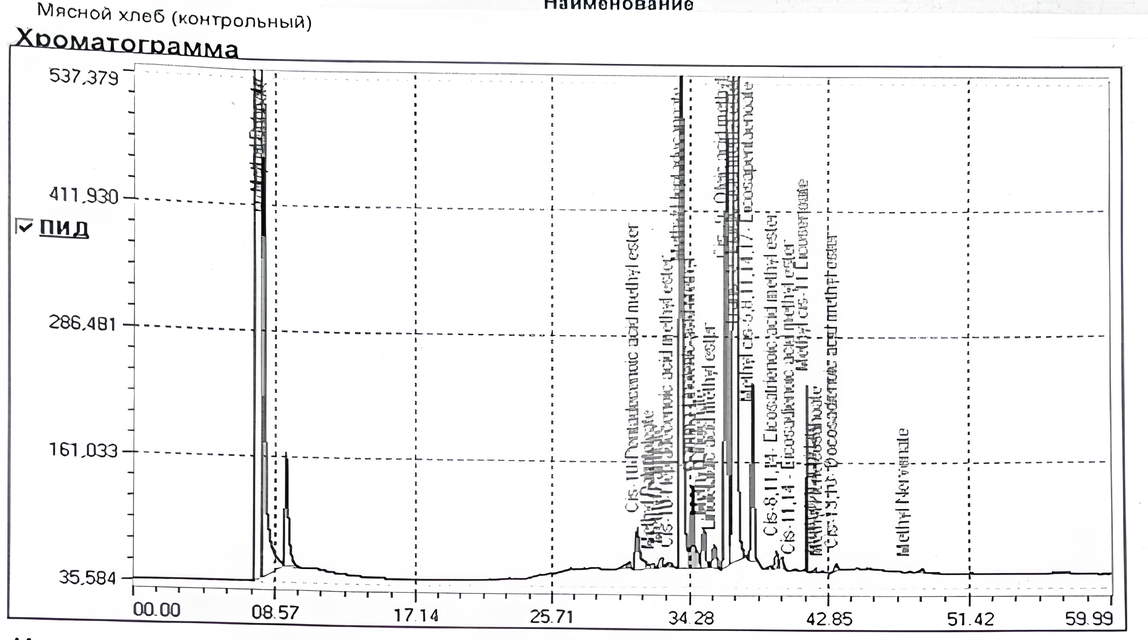
\includegraphics[width=0.8\textwidth]{media/pish2/image73}
	\caption*{}
\end{figure}


{\bfseries Рис.2 - Жирнокислотный состав контрольного образца мясного
хлеба}


\begin{figure}[H]
	\centering
	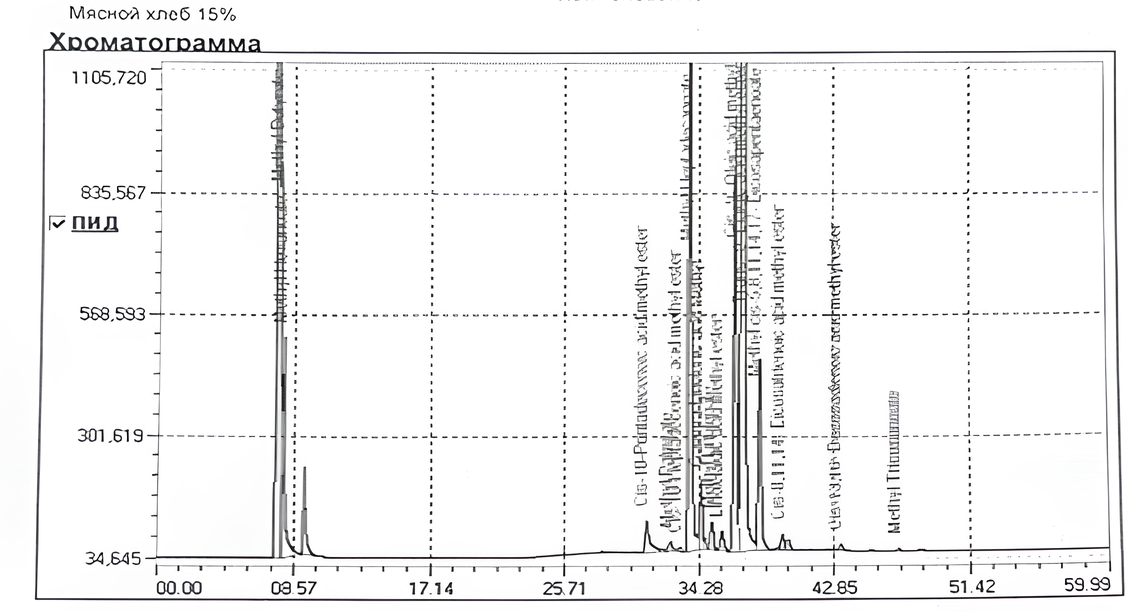
\includegraphics[width=0.8\textwidth]{media/pish2/image74}
	\caption*{}
\end{figure}


{\bfseries Рис.3 - Жирнокислотный состав образца мясного хлеба с 15\% ПТЖ}

Метилбутират и метилгексаноат, относящиеся к коротко- и среднецепочечным
метиловым эфирам, снизились в опытном образце в 1,36 и 1,45 раза
соответственно. Это свидетельствует об изменении состава летучих
соединений, что может оказывать влияние на ароматические характеристики
мясного хлеба, снижая сливочные нотки и усиливая растительные оттенки.

Содержание метилпальмитата (насыщенная жирная кислота) в
экспериментальном образце увеличилось в 2,18 раза, что может
способствовать повышению структурной стабильности продукта. Увеличение
количества метиловых эфиров цис-10-пентадеценовой и
цис-10-гептадекановой кислот в 2 и 2,5 раза соответственно указывает на
поступление в систему специфических растительных липидов из томатных
семян, характерных для растительных масел и морепродуктов.

Особое внимание заслуживает рост содержания полиненасыщенных жирных
кислот (ПНЖК). Концентрация метилового эфира γ-линоленовой кислоты
увеличилась в 2,45 раза, а метиллинолената -- в 1,6 раза, что
свидетельствует об обогащении мясного хлеба ценными омега-6 и омега-3
жирными кислотами, участвующими в регуляции липидного обмена и
обладающими противовоспалительными свойствами.

Отмечено значительное увеличение транс-9-элаидиновой кислоты
(транс-изомера олеиновой кислоты) в 2,86 раза, что, вероятно, связано с
термической обработкой продукта. В то же время содержание
цис-9-олеиновой кислоты, основной мононенасыщенной жирной кислоты,
увеличилось в 2,4 раза, что может способствовать улучшению усвояемости
жиров.

Значительное повышение уровня длинноцепочечных ПНЖК, таких как
эйкозапентаеновая (EPA) и эйкозатриеновая кислоты, указывает на
увеличение доли омега-3 жирных кислот в липидном профиле мясного хлеба.
Кроме того, концентрация цис-13,16-докозадиеновой кислоты возросла на
76\%, что подчеркивает ее участие в регуляции липидного обмена.

Таким образом, введение 15\% ПТЖ способствует увеличению содержания
полиненасыщенных жирных кислот (омега-3 и омега-6), мононенасыщенных
жирных кислот и специфических растительных липидов, что повышает
биологическую ценность и функциональные свойства мясного хлеба.

{\bfseries Выводы.} Результаты исследования подтверждают перспективность
обогащения мясного хлеба порошком из томатного жмыха (ПТЖ). Оптимальный
уровень добавления -- 15\%, поскольку он улучшает органолептические
характеристики продукта: придает ему насыщенный красновато-коричневый
оттенок благодаря природным пигментам томатов, делает консистенцию более
плотной за счет влагопоглощающих свойств клетчатки и формирует
сбалансированный вкус с умеренными томатными, фруктово-растительными и
ореховыми нотами. При этом снижается выраженность мясного и сливочного
вкуса, что связано с уменьшением концентрации метилбутирата и
метилгексаноата.

Добавление ПТЖ также приводит к изменению липидного профиля мясного
хлеба: повышается содержание ненасыщенных жирных кислот, включая омега-3
и омега-6, и снижается уровень насыщенных жиров. Это соответствует
современным требованиям к функциональным продуктам, способствующим
профилактике метаболических заболеваний.

Таким образом, использование ПТЖ в мясных изделиях повышает их пищевую
ценность, улучшает сенсорные свойства и способствует рациональному
использованию побочных продуктов пищевой промышленности, что делает
производство более экологически устойчивым. Полученные результаты могут
быть полезны при разработке новых рецептур функциональных мясных
продуктов с улучшенными липидными характеристиками и повышенной
привлекательностью для потребителей.

{\bfseries Литература}

1. Stangierski J.\&Lesnierowski G. Nutritional and health-promoting
aspects of poultry meat and its processed products //
World' s Poultry Science Journal. - 2015.-71(1).-
P.71-82. DOI
\href{http://dx.doi.org/10.1017/S0043933915000070}{10.1017/S0043933915000070}.

2. Zinina O., Merenkova S., Tazeddinova D., Rebezov M., Stuart M.,
Okuskhanova E.,Yessimbekov Zh. \& Baryshnikova, N. Enrichment of meat
products with dietary fibers: a review // Agronomy Research. -2020. - 17
(14).- P.387-396. DOI 10.15159/AR.19.163.

3. Functional Food Ingredients Market.
\url{https://www.maximizemarketresearch.com/market-report/global-functional-food-market/101443/.-}
Date of access: 18.12.2024

4. BrighinaS.,Pulvirenti L.,Siracusa L., Arena E.,Faulisi M.V.,Restuccia
C. Small-Sized Tomato Pomace: Source of Bioactive Compounds and
Ingredient for Sustainable Production of Functional Bread. // Foods -
2024. - 13(21).- P.3492. DOI 10.3390/foods13213492

5. Domínguez R., Gullón P., Pateiro M., Munekata P.WangangZ.\& Lorenzo
J. M., Tomato as Potential Source of Natural Additives for Meat Industry
// A Review. Antioxidants. -2020. - 9 (1). -P.73.
DOI10.3390/antiox9010073.

6. Lyu X., Ying D., Zhang P.~Effect of Whole Tomato Powder or Tomato
Peel Powder Incorporation on the Color, Nutritional, and Textural
Properties of Extruded High Moisture Meat Analogues // Food Bioprocess
Technol. -2024.~-17. -P.231-244.
\href{https://doi.org/10.1007/s11947-023-03133-x}{DOI
10.1007/s11947-023-03133-x}.

7. Ahmad U., Mushtaq Z., Ahmad R.S. and Asghar N. Characterization,
oxidative perspectives and consumer acceptability of tomato waste powder
supplemented cookies // The Journal of Animal \& Plant Sciences. - 2017.
- 27(6). -P.2045-2055.

8. Incoronato AL., Conte A., Gammariello D., Del Nobile MA. Meatloaf
with Semi-dry Vegetables: A Study of Processing and Preservation. //
Journal Food Process Technol. -2015. -6(8). -P.470. DOI
10.4172/2157-7110.1000470.

9. Islamova G.,UtebaevaА., ShingisovА. Study of physico-chemical
indicators and mineral composition of tomato pomace for enrichment of
meat products //BULLETIN of the Korkyt Ata Kyzylorda University.
-2024.-1(68).- P.186-195. DOI 10.52081/bkaku.2024.v68.i1.141.

10. SlavišaS.,Skwarek P.,Đurđević S., Karwowska M.,Pisinov B.,Tomasevic
I.,KurćubićV. Tomato Pomace Powder as a Functional Ingredient in Minced
Meat Products--- Influence on Technological and Sensory Properties of
Traditional Serbian Minced Meat Product Cevapi// Processes.
-2024.-12(7), -P.1330. DOI 10.3390/pr12071330.

11. Ahmad M., Qureshi S., Akbar M.H., Siddiqui S.A., Gani A., Mushtaq
M., et al. Plant-based meat alternatives: compositional analysis,
current development and challenges. // Applied Food Research. -2022. -
Vol.2 (2). - 100154. DOI 10.1016/j.afres.2022.100154.

\emph{{\bfseries Информация об авторах}}

Шингисов А. У. -доктор технических наук, профессор, член-корреспондент
Академии сельскохозяйственных наук Республики Казахстан и Академии
естественных наук Российской Федерации, Южно-Казахстанский университет
им. М.Ауэзова, Шымкент, Қазақстан, e- mail: azret\_utebai@mail.ru;

Утебаева А.А. - PhD доктор, Южно-Казахстанский университет им.
М.Ауэзова, Шымкент, Қазақстан, e- mail: aidana.utebaeva@gmail.com;

Исламова Г.Е.- докторант, Южно-Казахстанский университет им. М.Ауэзова,
Шымкент, Қазақстан, e- mail: Gulnura\_87\_KZ@mail.ru

\emph{{\bfseries Information about the authors}}

Shingisov A.U.- doctor of Technical Sciences., professor, Corresponding
Member of the Academy of Agricultural Sciences of the Republic of
Kazakhstan and the Academy of Natural Sciences of the Russian
Federation, South Kazakhstan University M. Auezov, Shymkent,
Kazakhstan,e- mail:
\href{mailto:azret_utebai@mail.ru}{\nolinkurl{azret\_utebai@mail.ru}};

Utebaeva A.A.- PhD, South Kazakhstan University M. Auezov, Shymkent,
Kazakhstan, e- mail: aidana.utebaeva@gmail.com;

Islamova G.E.- doctoral student, South Kazakhstan University M.
Auezov,Shymkent, Kazakhstan, e- mail: Gulnura\_87\_KZ@mail.ru\
